% File that compiles all other files into one clean document.

%Layout, imports, packages, class
%%%%%%%%%%%%%%%%%%%%%%%%%%%%%%%%%%%%%%%%%%%%%%%%%%
% PAGE LAYOUT
%%%%%%%%%%%%%%%%%%%%%%%%%%%%%%%%%%%%%%%%%%%%%%%%%%
\documentclass[a4paper,11pt]{report}
%\usepackage[subtle]{savetrees}
\usepackage{fullpage}
\usepackage{wrapfig}
%%%%%%%%%%%%%%%%%%%%%%%%%%%%%%%%%%%%%%%%%%%%%%%%%%
%% PAGEHEADER STYLING
%%%%%%%%%%%%%%%%%%%%%%%%%%%%%%%%%%%%%%%%%%%%%%%%%%
\usepackage{etoolbox,fancyhdr,xcolor}
%%%%%%%%%%%%%%%%%%%%%%%%%%%%%%%%%%%%%%%%%%%%%%%%%%
% EXTERNAL INCLUDES
%%%%%%%%%%%%%%%%%%%%%%%%%%%%%%%%%%%%%%%%%%%%%%%%%%
\usepackage{graphicx}
\usepackage{svg}
\usepackage{csvsimple}
\usepackage{pdfpages}
\usepackage{hyperref}
\usepackage{lscape}
\usepackage{eurosym}
%%%%%%%%%%%%%%%%%%%%%%%%%%%%%%%%%%%%%%%%%%%%%%%%%%
%% BIBLIOGRAPHY SETTINGS
%%%%%%%%%%%%%%%%%%%%%%%%%%%%%%%%%%%%%%%%%%%%%%%%%%
\usepackage[comma]{natbib}
\usepackage{color, colortbl}
\usepackage[nonumberlist,acronym]{glossaries}
%%%%%%%%%%%%%%%%%%%%%%%%%%%%%%%%%%%%%%%%%%%%%%%%%%
% CAPTIONS AND REFERENCING
%%%%%%%%%%%%%%%%%%%%%%%%%%%%%%%%%%%%%%%%%%%%%%%%%%
\usepackage{fancyref}
%\usepackage{image_captioning}
%%%%%%%%%%%%%%%%%%%%%%%%%%%%%%%%%%%%%%%%%%%%%%%%%%
%% CODE SNIPPET LISTING SETTINGS
%%%%%%%%%%%%%%%%%%%%%%%%%%%%%%%%%%%%%%%%%%%%%%%%%%
\usepackage{listings}
\renewcommand\lstlistlistingname{List of Listings}
\lstset{numbers=left,xleftmargin=2em,captionpos=b}
%%%%%%%%%%%%%%%%%%%%%%%%%%%%%%%%%%%%%%%%%%%%%%%%%%
%    SECTIONS
%%%%%%%%%%%%%%%%%%%%%%%%%%%%%%%%%%%%%%%%%%%%%%%%%%
\usepackage{titlesec}
\usepackage{sectsty}
\usepackage{csquotes}
%%%%%%%%%%%%%%%%%%%%%%%%%%%%%%%%%%%%%%%%%%%%%%%%%%
%% APPENDIX SETTINGS
%%%%%%%%%%%%%%%%%%%%%%%%%%%%%%%%%%%%%%%%%%%%%%%%%%
\usepackage[titletoc]{appendix}
%\renewcommand\appendixtocname{Appendices}
%\renewcommand\appendixpagename{Appendices}
%All non-canonical parts/chapters should be numbered with roman numbers
\pagenumbering{roman}
\pdfminorversion=7

%Titlepage
\title{Software Requirements Specification \\
for \\
Warehouse Drone Collision Avoidance Project}
\author{Prepared by Tristan van Vegchel \\
Seacon Logistics \\
Approved from version 1.0 onwards}
\date{Venlo, created on November 11, 2019}

%glossaries
\makenoidxglossaries
%File for glossaries

%Glossaries
\newglossaryentry{OpenCV}
{
	name={OpenCV},
	description={OpenCV (Open Source Computer Vision Library) is an open source computer vision and machine learning software library. OpenCV was built to provide a common infrastructure for computer vision applications and to accelerate the use of machine perception in the commercial products. Being a BSD-licensed product, OpenCV makes it easy for businesses to utilize and modify the code} \cite{About_OpenCv}
}

\newglossaryentry{Artificial Intelligence}
{
	name={Artificial Intelligence},
	description={The theory and development of computer systems able to perform tasks normally requiring human intelligence, such as visual perception, speech recognition, decision-making, and translation between languages}
}

\newglossaryentry{deep learning}
{
	name={Deep Learning},
	description={A subset of machine learning in artificial intelligence that makes use of artificial neural networks.}
}

%Abbreviations
\newacronym{STG2}{STG2}{Graduation Project}
\newacronym{AI}{A.I.}{Artificial Intelligence}
\newacronym{FHTenL}{Fontys}{Fontys University of Applied Sciences}
\newacronym{KPI}{KPI}{Key Performance Indicators}
\newacronym{TBD}{TBD}{To Be Determined}
\newacronym{RACI}{RACI matrix}{Responsible-Accountable-Consulted-Informed matrix}
\setacronymstyle{long-short}


%\printnoidxglossary[title=Definitions]

%Bibliography
\renewcommand{\bibname}{References}


%Put includes in document environment
\begin{document}
	\maketitle
	\setcounter{page}{2}
	
	%Information page
	%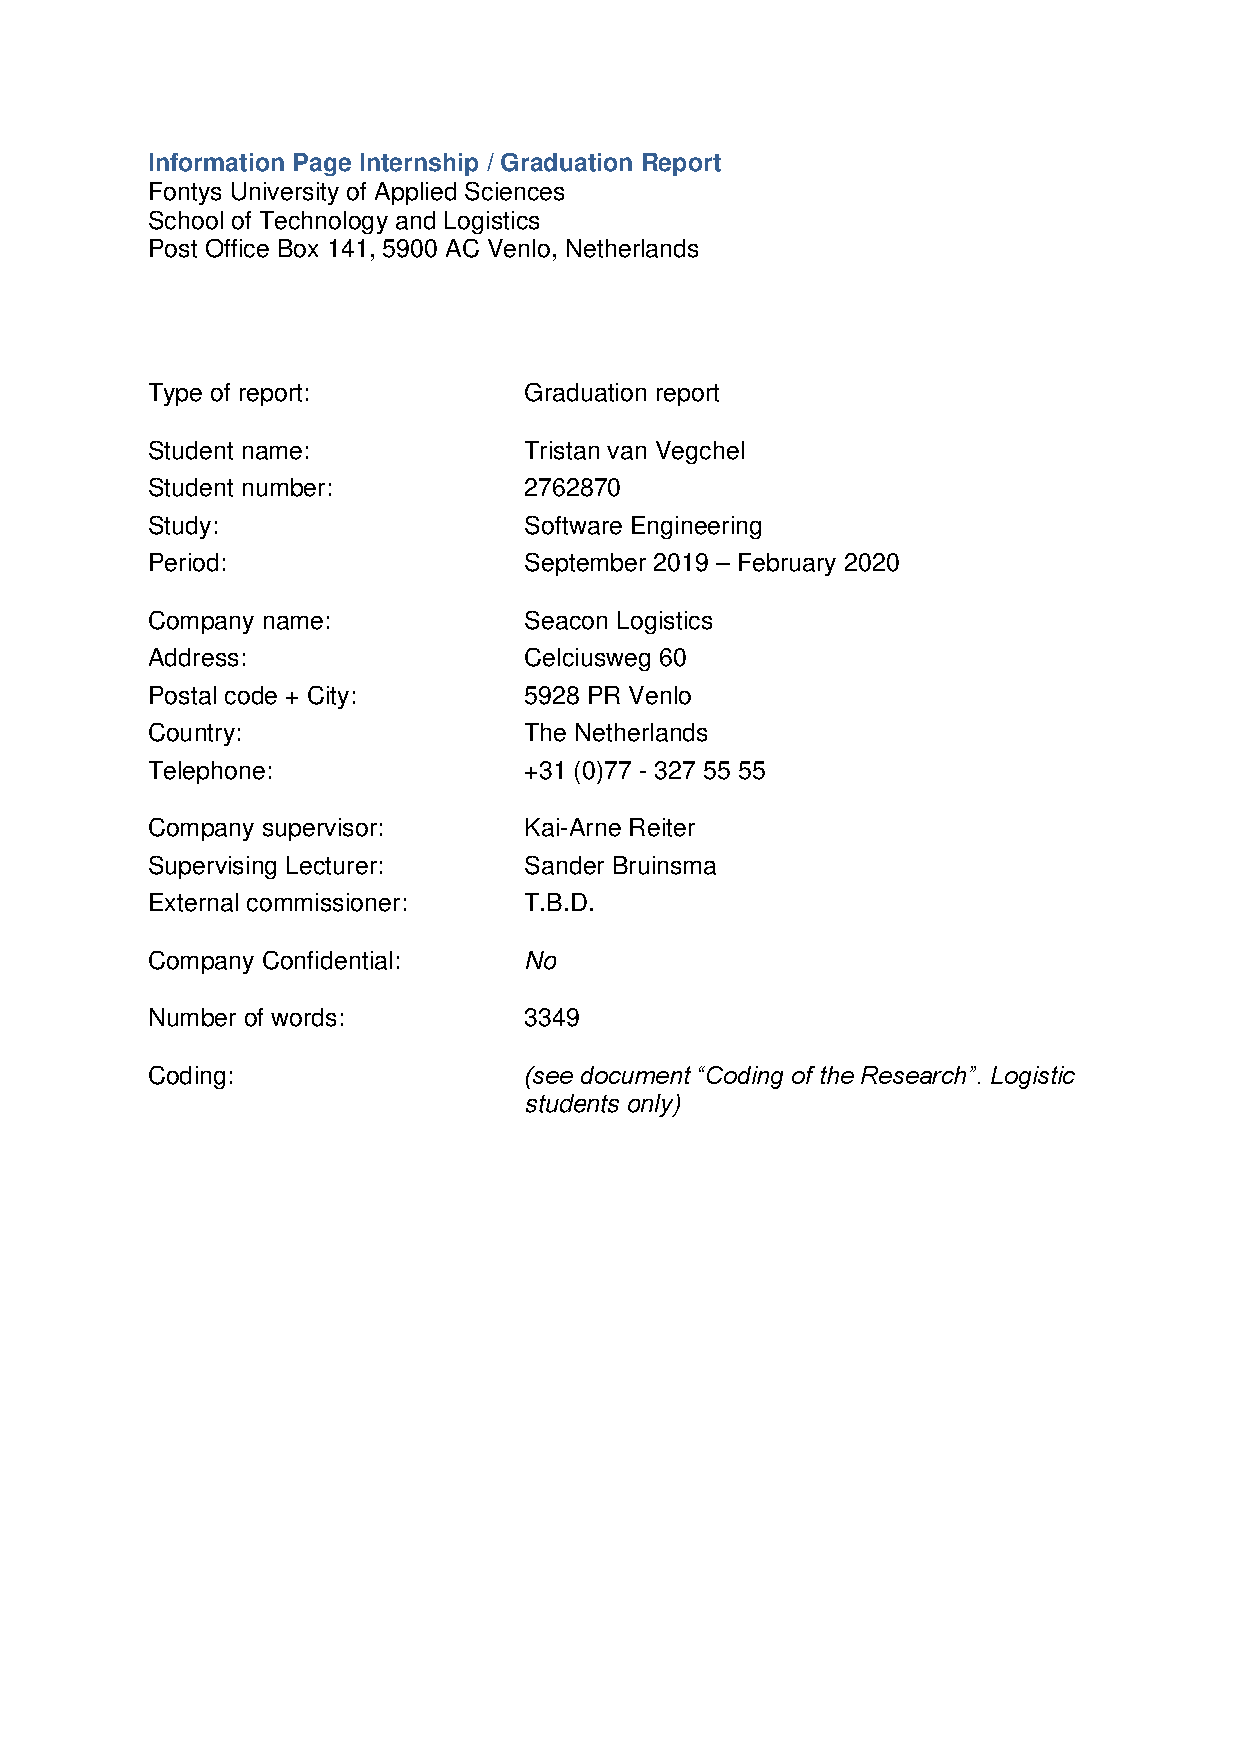
\includepdf[pagecommand={}]{utility/InformationPage}
	
	%Abstract
	%\noindent
The warehouse drone collision avoidance project concerns itself with the analysis, design, and development of a solution to provide a drone with collision avoidance functionality. The time scope was set for 1 semester (5 months), and resulted in the creation of this bachelor thesis. This project contains 2 prototype concepts: A concept based on reinforcement learning and a concept based on combining computer vision with a state machine implementation. The reinforcement learning concept did not show promising results as it did not show any sign of learning. The state machine concept its components work separately, but still requires smoother transitioning and a number of bugs needed to be fixed before it is able to run the entire state machine properly. This project also contained a research aspect. This research focused on the viability of Artificial Intelligence techniques for collision avoidance. Out of this came 3 approaches, of which one was created a prototype for. From the research it can be concluded that a single, stand-alone reinforcement learning algorithm is insufficient when attempting to use drones for cycle counting.
	
	%Statement of authenticity
	%
\includepdf[pagecommand={}]{utility/Statement_of_Authenticity}
	
	%%%%%%%%%%%%%%%%%%%%%%%%%%%%%%%%%%%%%%%%%%%%%%%%%%
%% CONFIGURATION OF PAGE HEADER
%%%%%%%%%%%%%%%%%%%%%%%%%%%%%%%%%%%%%%%%%%%%%%%%%%
\pagestyle{fancy}
\newcommand{\headrulecolor}[1]{\patchcmd{\headrule}{\hrule}{\color{#1}\hrule}{}{}}
\newcommand{\footrulecolor}[1]{\patchcmd{\footrule}{\hrule}{\color{#1}\hrule}{}{}}
\pagestyle{fancy}
\fancyhf{}% Clear header/footer
\fancyhead[C]{}
\fancyhead[R]{\thepage}
\setlength{\headsep}{33pt}
\setlength{\headheight}{13.6pt}
\renewcommand{\headrulewidth}{0.4pt}
\setlength{\parindent}{0em}
	%Content display
	\tableofcontents
	\listoffigures
	
	%Version history
	\pagebreak
	%\vhListAllAuthorsLong
	%Author macros
	\newcommand{\TVV}{Tristan van Vegchel}
	\renewcommand \vhAuthorColWidth{.7\hsize}
	\renewcommand \vhChangeColWidth{1.3\hsize}
	\begin{versionhistory}
		\vhEntry{0.1}{11-11-2019}{\TVV}{Created skeleton}
		\vhEntry{0.1}{12-11-2019}{\TVV}{Created shortened version}
		\vhEntry{0.2}{27-11-2019}{\TVV}{Added introduction}
		\vhEntry{0.3}{06-12-2019}{\TVV}{Added overall description}
		\vhEntry{0.4}{23-12-2019}{\TVV}{Added functional requirements}
		\vhEntry{0.5}{01-01-2020}{\TVV}{Completed first draft}
		\vhEntry{1.0}{10-01-2020}{\TVV}{Document reviewed and approved}
	\end{versionhistory}
	\glsaddall
	\printnoidxglossary[type=\acronymtype,title=List of Abbreviations]
	\printnoidxglossary[title=Definitions]
	
	%Main part
	\pagebreak
	\pagenumbering{arabic}
	
	\chapter{Introduction}
\lhead{\thechapter \space Introduction}
\label{ch:introduction}

\section{Purpose}
%TO DO: Identify the product for which this document is written, as well as the intended audience
The purpose of this document is to provide a detailed description of the software product of the Drone Warehouse Collision Avoidance project. It contains the purpose and features of the software, the interfaces, and the constraints under which it must operate. This document is primarily intended for the department of Engineering \& IT of Seacon Logistics, as this department will contain/contains the future developers of the next iteration of this product. As this project is developed as a bachelor thesis project, the by Fontys University of Applied Sciences appointed tutors, lecturers, and experts are also considered an intended audience.

\section{Document Conventions \& Standards}
%TO DO: Describe any naming or typographical conventions, as well as the standards used (IEEE). For example, state whether priorities  for higher-level requirements are assumed to be inherited by detailed requirements, or whether every requirement statement is to have its own priority.
This document was created based on the IEEE Recommended Practice for Software Requirement Specifications standard 830-1998.

\section{Scope}
%TO DO: Summarize each of the named software products, including what they will and won't do. Also describe the application of the software, such as what the benefits, objectives, and or goals are.
The Warehouse Drone Collision Avoidance system (which is in this document generally referred to as "product") will primarily be responsible for providing a drone with a prototype solution to move along all layers of a single side of a rack in a warehouse, while avoiding collisions.

\section{Overview}
%TODO: List what the rest of this document will contain, and in what order.
The remainder of this document will feature an overall description of the product and the specific requirements. The former includes the perspective, information regarding a set of used interfaces, the product functions, and information regarding the product its users. The latter contains the specific requirements listed with unique identifiers, and a list of assumptions made in order for the product to function.


	\chapter{Overall Description}
\lhead{\thechapter \space Overall Description}
\label{ch:overall_description}

\section{Product Perspective}
%TO DO: Explain whether or not the product is part of a larger system. In case it is, explain how this product will contribute to the larger system's requirements and identify interfaces between this product and the rest of the system. Using diagrams to elaborate is helpful
The product will be developed as a first step of a larger project, which ultimately has the goal to semi-automate the cycle count processes of the inventory control \& management department of the customer's warehouses. The concept was initially developed in order to combat the increasing scarceness of warehouse cycle count employees. An overview of the larger project can be found in figure \ref{fig:roadmap}.

\paragraph{System Interfaces}
As the product for which this document is written will be the first component of the Seacon Drone project, the interfaces of the Seacon Drone project which the product will communicate with have yet to be defined.

\paragraph{Hardware Interfaces}
The product will support Dji Tello drones \citep{tello}. It will developed to be used with a Wi-Fi enabled laptop. The product will provide a set of drone control command keys, which will only work as intended on an QWERTY or AZERTY keyboard layout.

\paragraph{Software Interfaces}
The product will be developed in Ubuntu 18.04. This will thus be the only operating system and version which will have guaranteed support. Furthermore, the device running the product is required to have a python interpreter version 3.6.x with pip, as this will be the language and package management system for development, respectively. The python-pip packages the software will make use of are:
\begin{itemize}
	\item opencv-python (version 4.1.1.26) \citep{opencv}
	\item av (version 6.2.0) \citep{av}
	\item tellopy (version 0.6.0) \citep{tellopy}
	\item simple\_pid (version 0.2.4) \citep{pid}
	\item pynput (version 1.4.5) \citep{pynput}
\end{itemize}

\begin{figure}[ht]
	\centering
	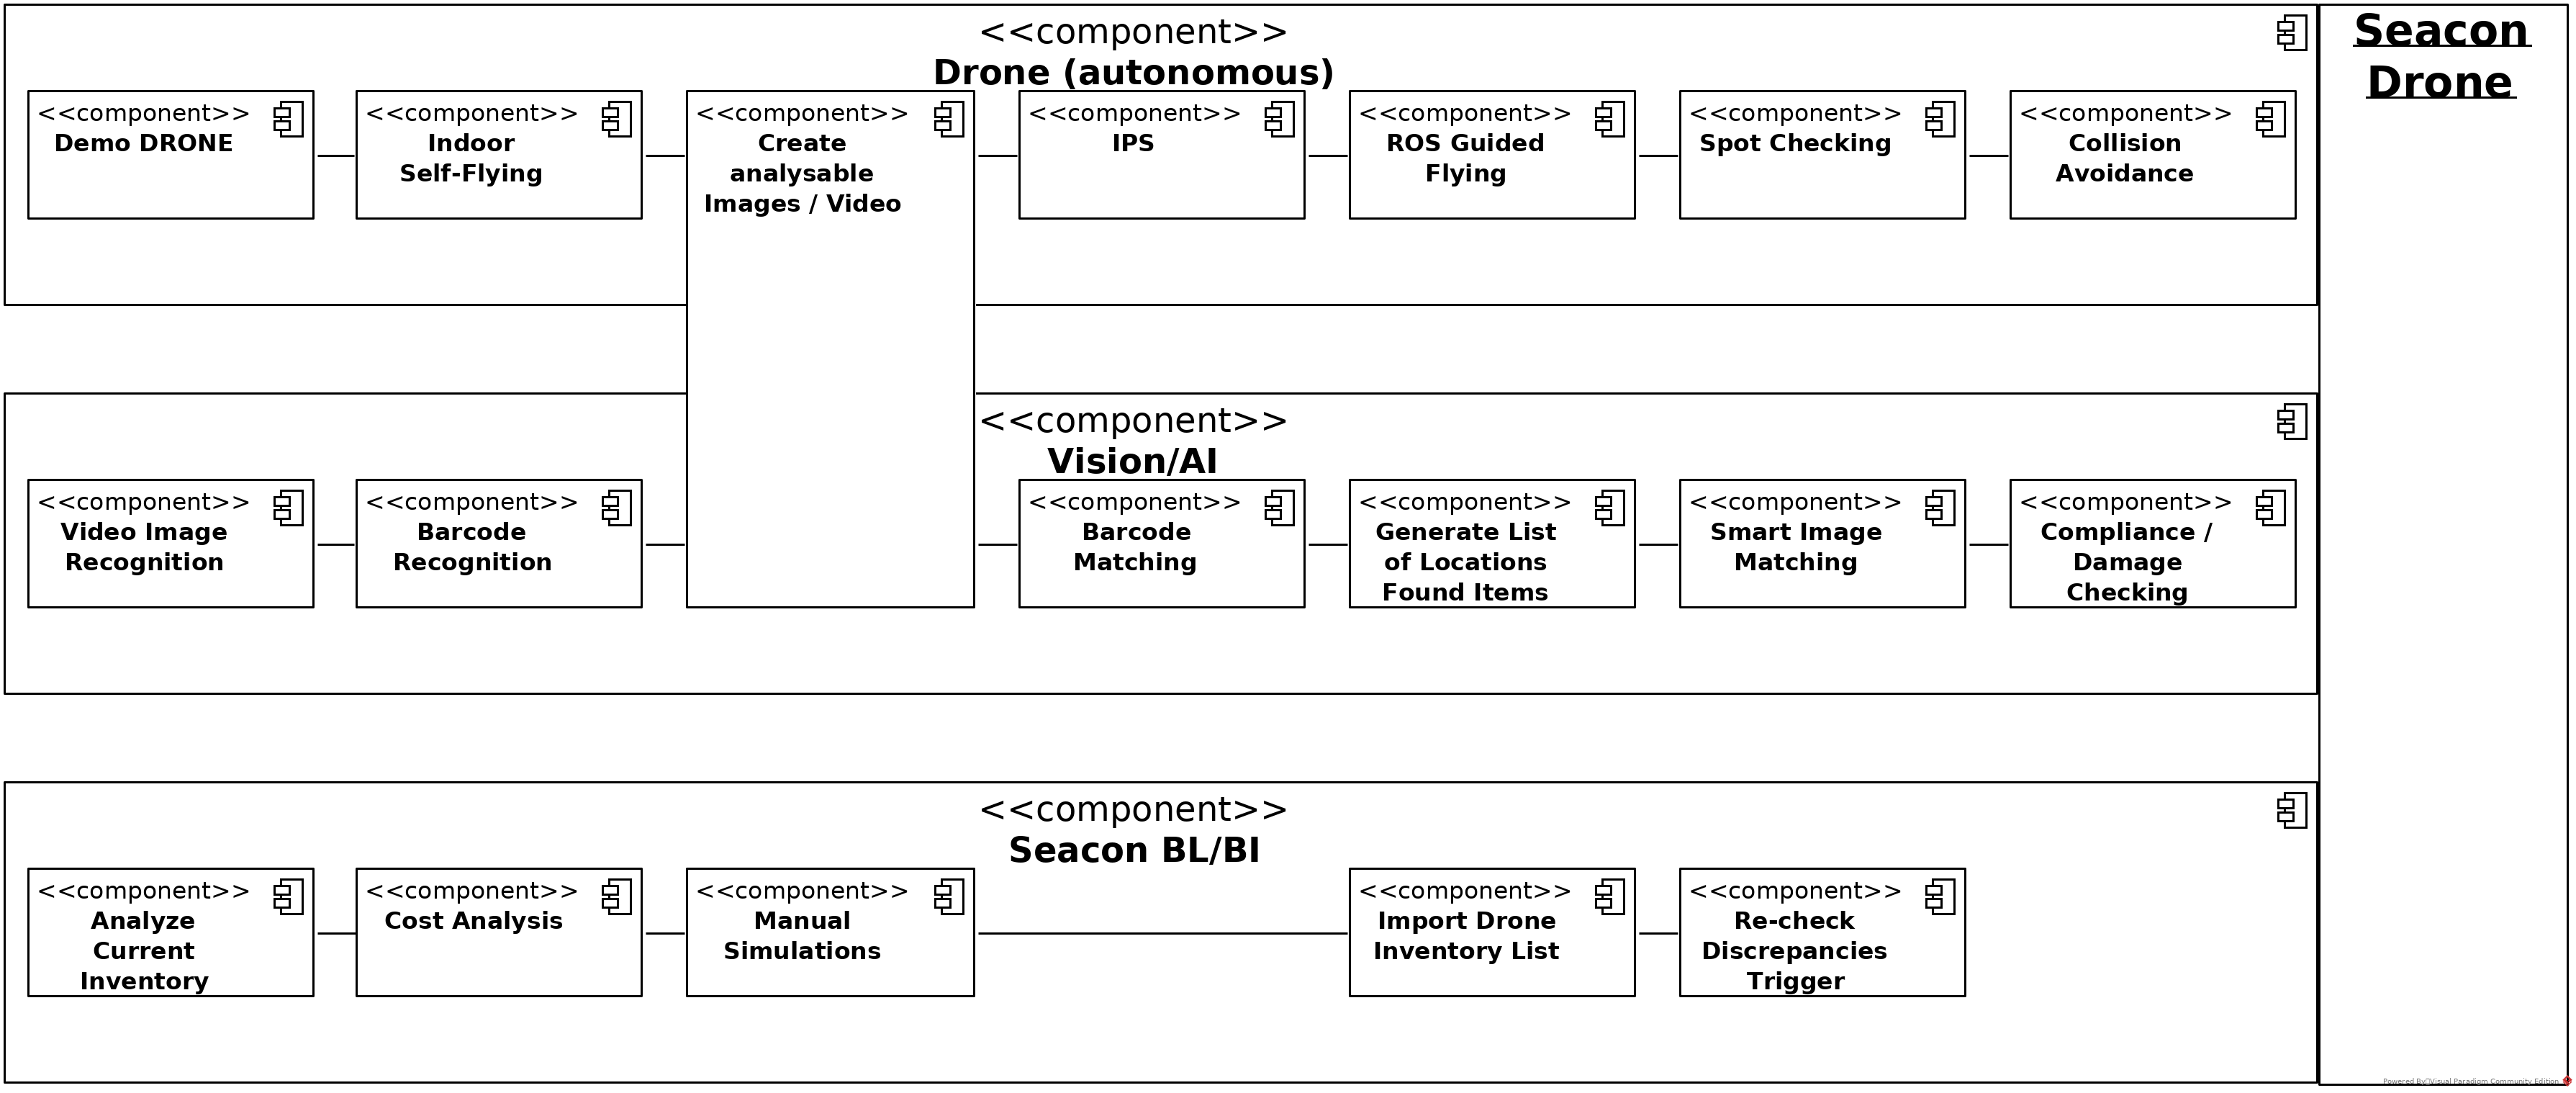
\includegraphics[width=\linewidth]{img/seacon_roadmap.png}
	\label{fig:roadmap}
	\caption{Roadmap of the Seacon Drone Project}
\end{figure}
\pagebreak
\section{Product Functions}
The product can be divided into 3 parts: x-axis, y-axis, z-axis of the drone. Each axis can then be subdivided further into a video processing part, drone movement part, and a collision avoidance part. Figure \ref{fig:drone_concept} visualizes those 3 axes.
\begin{figure}[h]
	\centering
	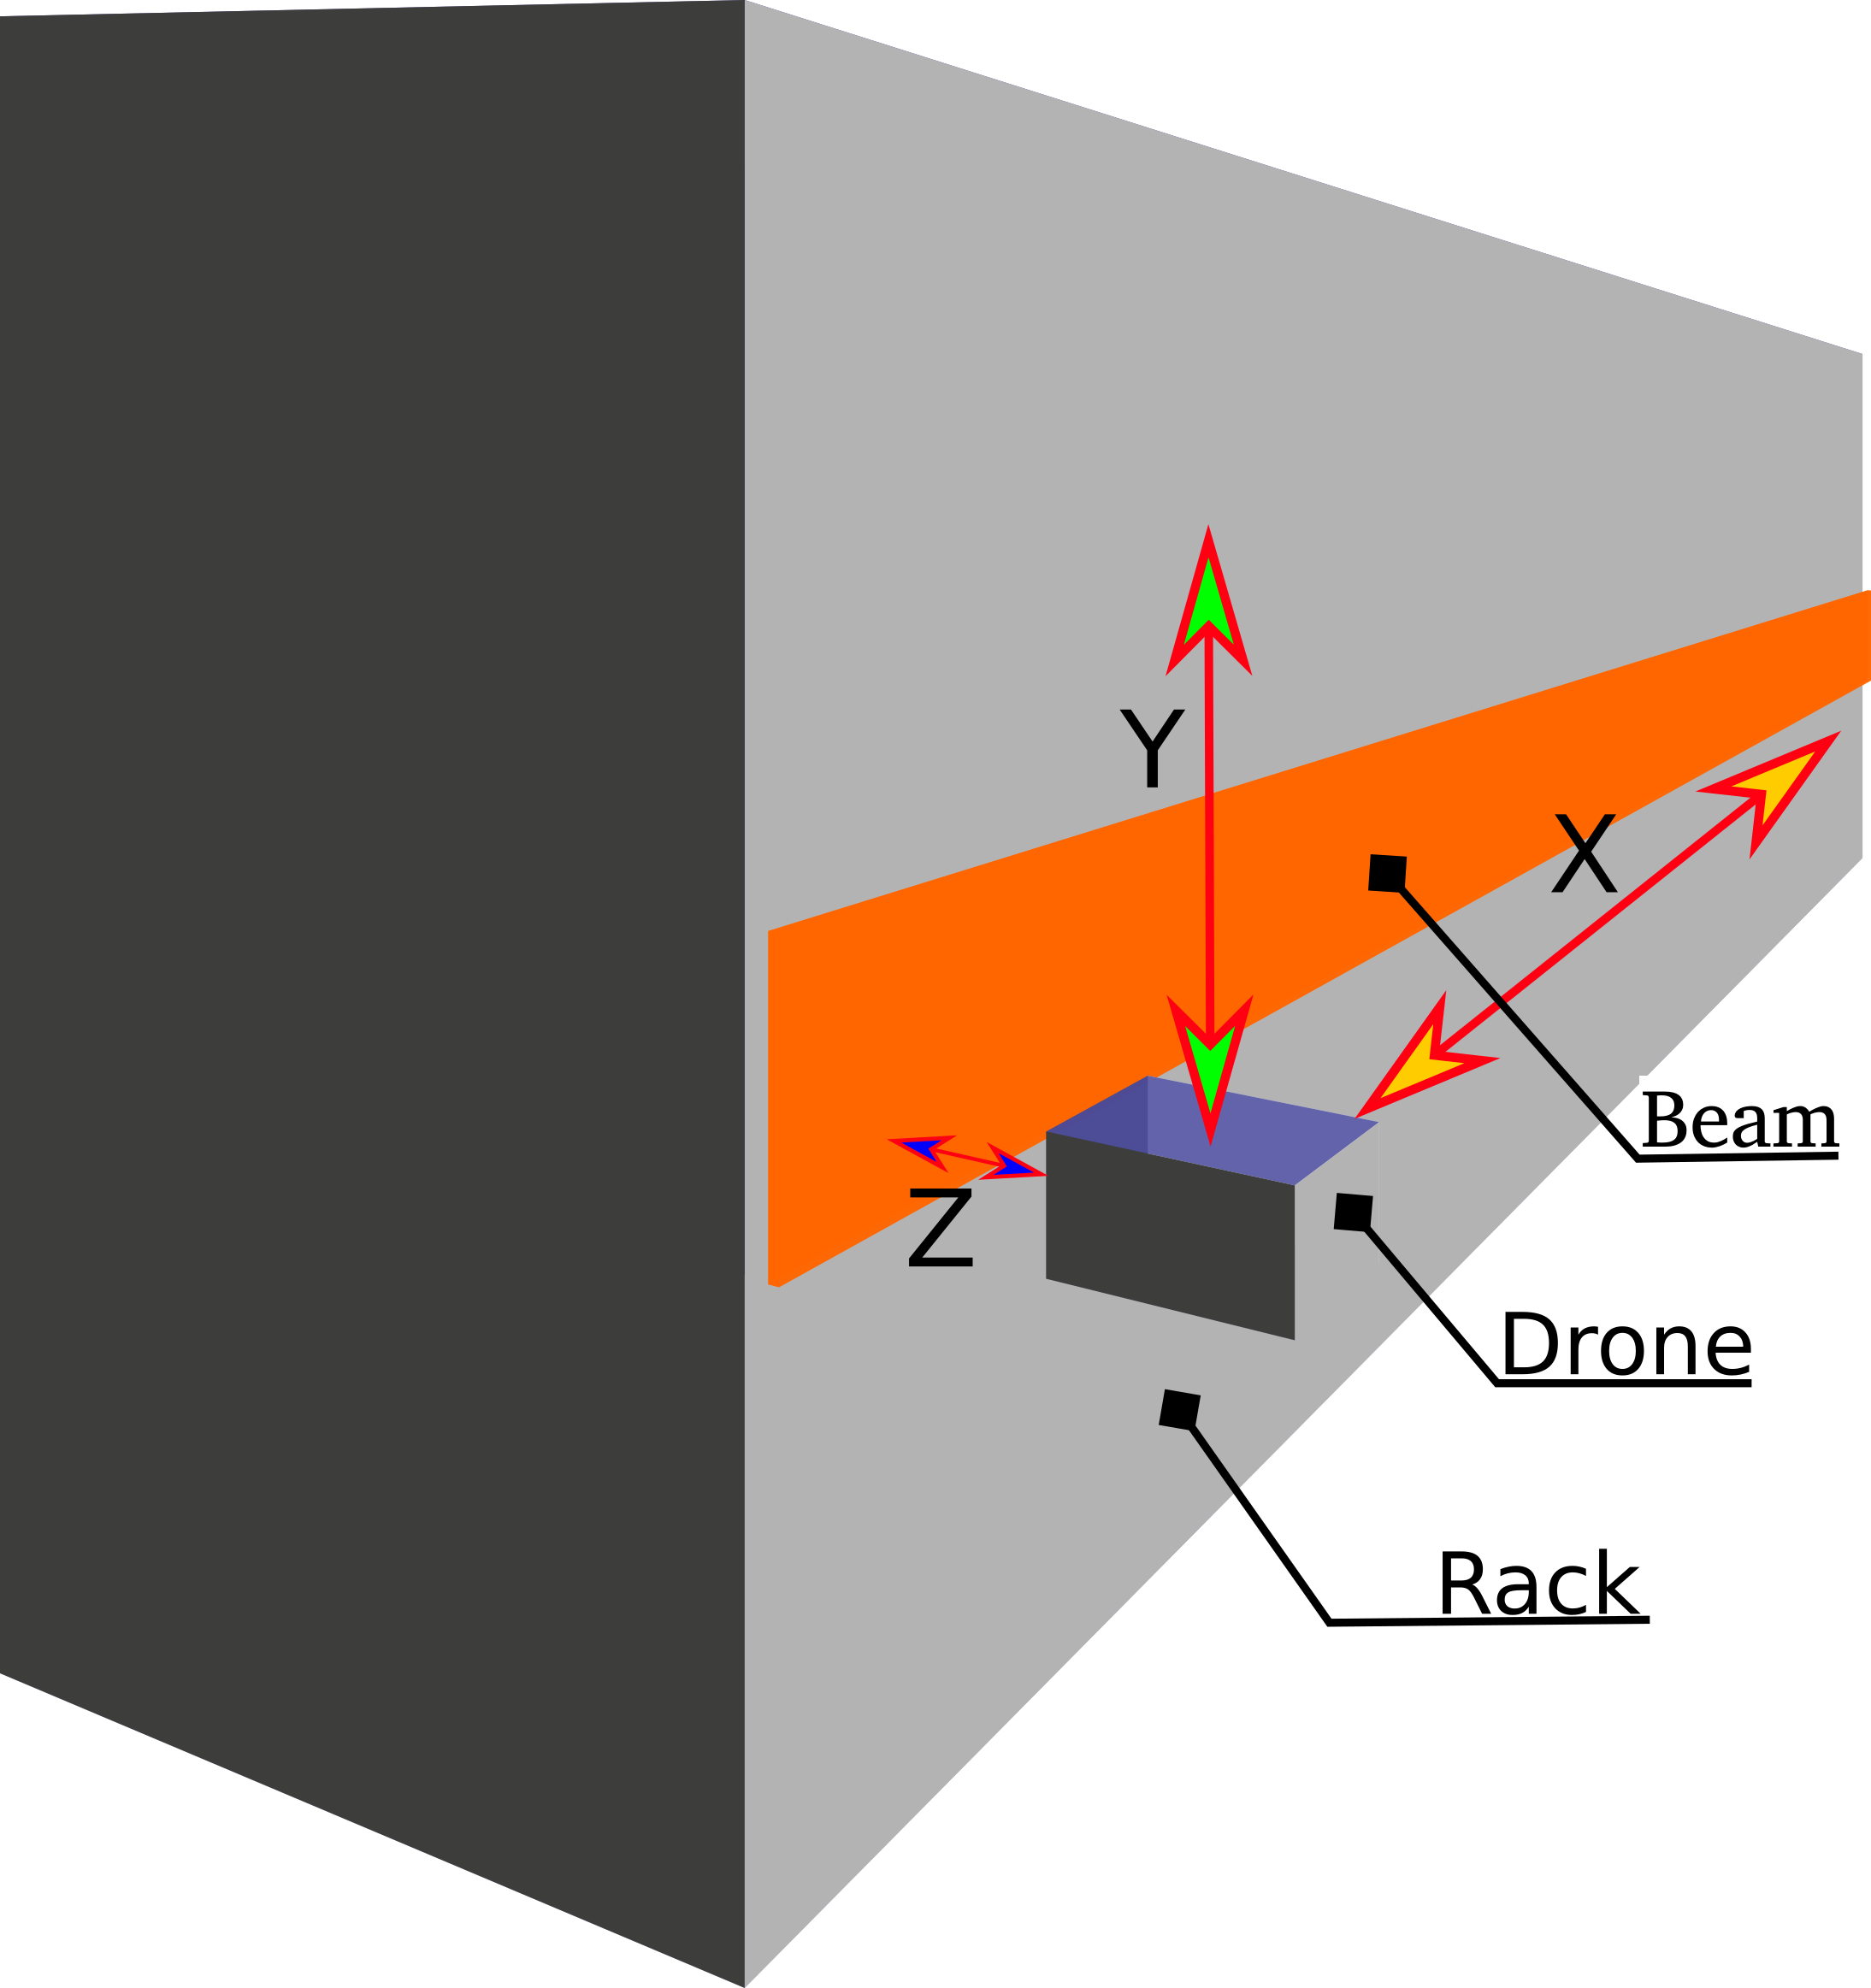
\includegraphics[width=\linewidth/2]{img/drone_concept_diagram.png}
	\label{fig:drone_concept}
	\caption{Simple drawing visualizing the intended product.}
\end{figure}
\pagebreak
\begin{itemize}
	\item X-axis:
	\begin{itemize}
		\itemsep0em
		\item Move the drone sideways
		\item Stop the drone at the end of a bar
		\item Detect objects in the drone's trajectory
		\item Avoid collisions with objects in the drone's trajectory
	\end{itemize}
	\item Y-axis:
	\begin{itemize}
		\itemsep0em
		\item Keep the bar in the center of the drone's camera
		\item Change the drone's altitude to switch layers
		\item Keep track of the current layer and the highest layer
	\end{itemize}
	\item Z-axis:
	\begin{itemize}
		\itemsep0em
		\item Estimate the pixel size of the bar
		\item Keep the drone to maintain distance from the bar
	\end{itemize}
\end{itemize}
When referring to "objects", one of the following things is meant:
\begin{itemize}
	\itemsep0em
	\item Pallets
	\item Racks
	\item Forklifts
	\item People
	\item Drones
\end{itemize}

\section{User Classes and Characteristics}
As the product of this iteration will not yet include inventory control functionality, the typical users do currently not include a warehouse employee class. Thus the sole user class of this product will be developers who aim to improve and/or extend the current product. Developers are required to have an extensive knowledge of Python and Opencv.



	\chapter{Specific Requirements}
\lhead{\thechapter \space Specific Requirements}
\label{ch:specific_requirements}

\section{Functional Requirements}
The following section describes the functions the product shall, should, and might include. For the definitions of these 3 terms refer to the glossary. Each of these 3 terms form a section, which are then further segmented into status, maintenance, and action tasks, for which the definitions can also be found in the glossary. Each functional requirement will have the following format:
\begin{figure}[h]
	\centering
	
\includegraphics[width=\linewidth]{img/func_req_format.png}
	\label{fig:func_req_format}
	\caption{Format for a functional requirement.}
\end{figure}

\noindent
Whereas:
\begin{itemize}
	\item \textbf{a} is the priority group (shall, should, might)
	\item \textbf{b} is the type of task
	\item \textbf{c} is the unique number of that requirement within its group.
\end{itemize}
Each requirement is prefixed by at least one set of brackets containing its unique ID, but may have a second set containing one or more IDs of prerequisite tasks or groups, each separated by comma. Note that in figure \ref{fig:func_req_format} the prerequisites bracket contains a single \textbf{"a"}, which indicates that all requirements in that priority group are a prerequisite to that task.\\\\

\textbf{[1] The product shall make the drone:}
\begin{itemize}
	\item \textbf{[1.1]} Status tasks:
	\begin{itemize}
		\item \textbf{[1.1.1]} Track the vertical center of the beam
		\item \textbf{[1.1.2]} Estimate the distance from the beam
		\item \textbf{[1.1.3]} Distinguish objects in the foreground from the background
		\item \textbf{[1.1.4]}[1.1.3, 1.2.1, 1.2.2] Check for objects in its trajectory
	\end{itemize}
	\item \textbf{[1.2]} Maintenance tasks:
	\begin{itemize}
		\item \textbf{[1.2.1]}[1.1.1] Maintain its altitude to keep the beam vertically centered
		\item \textbf{[1.2.2]}[1.1.2] Maintain a distance between 30 - 80 centimeters from the beam
	\end{itemize}
	\item \textbf{[1.3]} Action tasks:
	\begin{itemize}
		\item \textbf{[1.3.1]}[1.2] Move along the beam from left to right
		\item \textbf{[1.3.2]}[1.1.4] Avoid collisions by landing
	\end{itemize}
\end{itemize}
\noindent
\textbf{[2] The product should make the drone:}
\begin{itemize}
	\item \textbf{[2.1]} Status tasks:
	\begin{itemize}
		\item \textbf{[2.1.1]} Keep track of the remaining layers needing to be scanned
		\item \textbf{[2.1.2]} Determine the end of the beam
	\end{itemize}
	\item \textbf{[2.3]} Action tasks:
	\begin{itemize}
		\item \textbf{[2.3.1]}[1.1.2, 2.1] Move to other layers of a rack
		\item \textbf{[2.3.2]}[1.2] Move along the beam from right to left
		\item \textbf{[2.3.3]}[2.1.2] Stop at the end of the beam
	\end{itemize}
\end{itemize}
\noindent
\textbf{[3] The product might make the drone:}
\begin{itemize}
	\item \textbf{[3.1]} Status tasks:
	\begin{itemize}
		\item \textbf{[3.1.1]}[1.1.4] Determine if an object in its trajectory can be avoided
		\item \textbf{[3.1.2]} Determine pixel size:distance ratio of the beam
		\item \textbf{[3.1.3]}[1.2.1] Detect bar-codes on the beam
	\end{itemize}
	\item \textbf{[3.2]} Maintenance tasks:
	\begin{itemize}
		\item \textbf{[3.2.1]}[3.1.1] Readjust trajectory to avoid collision
	\end{itemize}
	\item \textbf{[3.3]} Action tasks:
	\begin{itemize}
		\item \textbf{[3.3.1]}[3.2.1] Move to the opposite rack of the same hallway
	\end{itemize}
	
\end{itemize}

\section{Assumptions}
In order for the product to function accordingly, the following assumptions have been made:
\begin{itemize}
	\itemsep0em
	\item The user is required to fly the drone to the correct starting position. This position is for the drone to face the left end of the lowest beam, at a distance between 30-80 centimeters.
	\item There are no things sticking out more than 10 centimeters from the rack.
	\item The drone will have enough battery capacity to complete one side of a rack.
	\item The warehouse interior lights are turned on and provide enough lighting.
	\item The drone is equipped with an RGB-camera.
	\item There is at least 3 meters of free space after the end of a beam.
	\item The drone remains connected to the device controlling it.
\end{itemize}
	
	%Bibliography
	\bibliographystyle{agsm}
	\bibliography{utility/bibliography}
	
	%Appendices
	%\begin{appendices}
		%\chapter{Drone States}
\lhead{\thechapter \space Drone States}
\label{app:drone_states}

\begin{figure}[h]
	\centering
	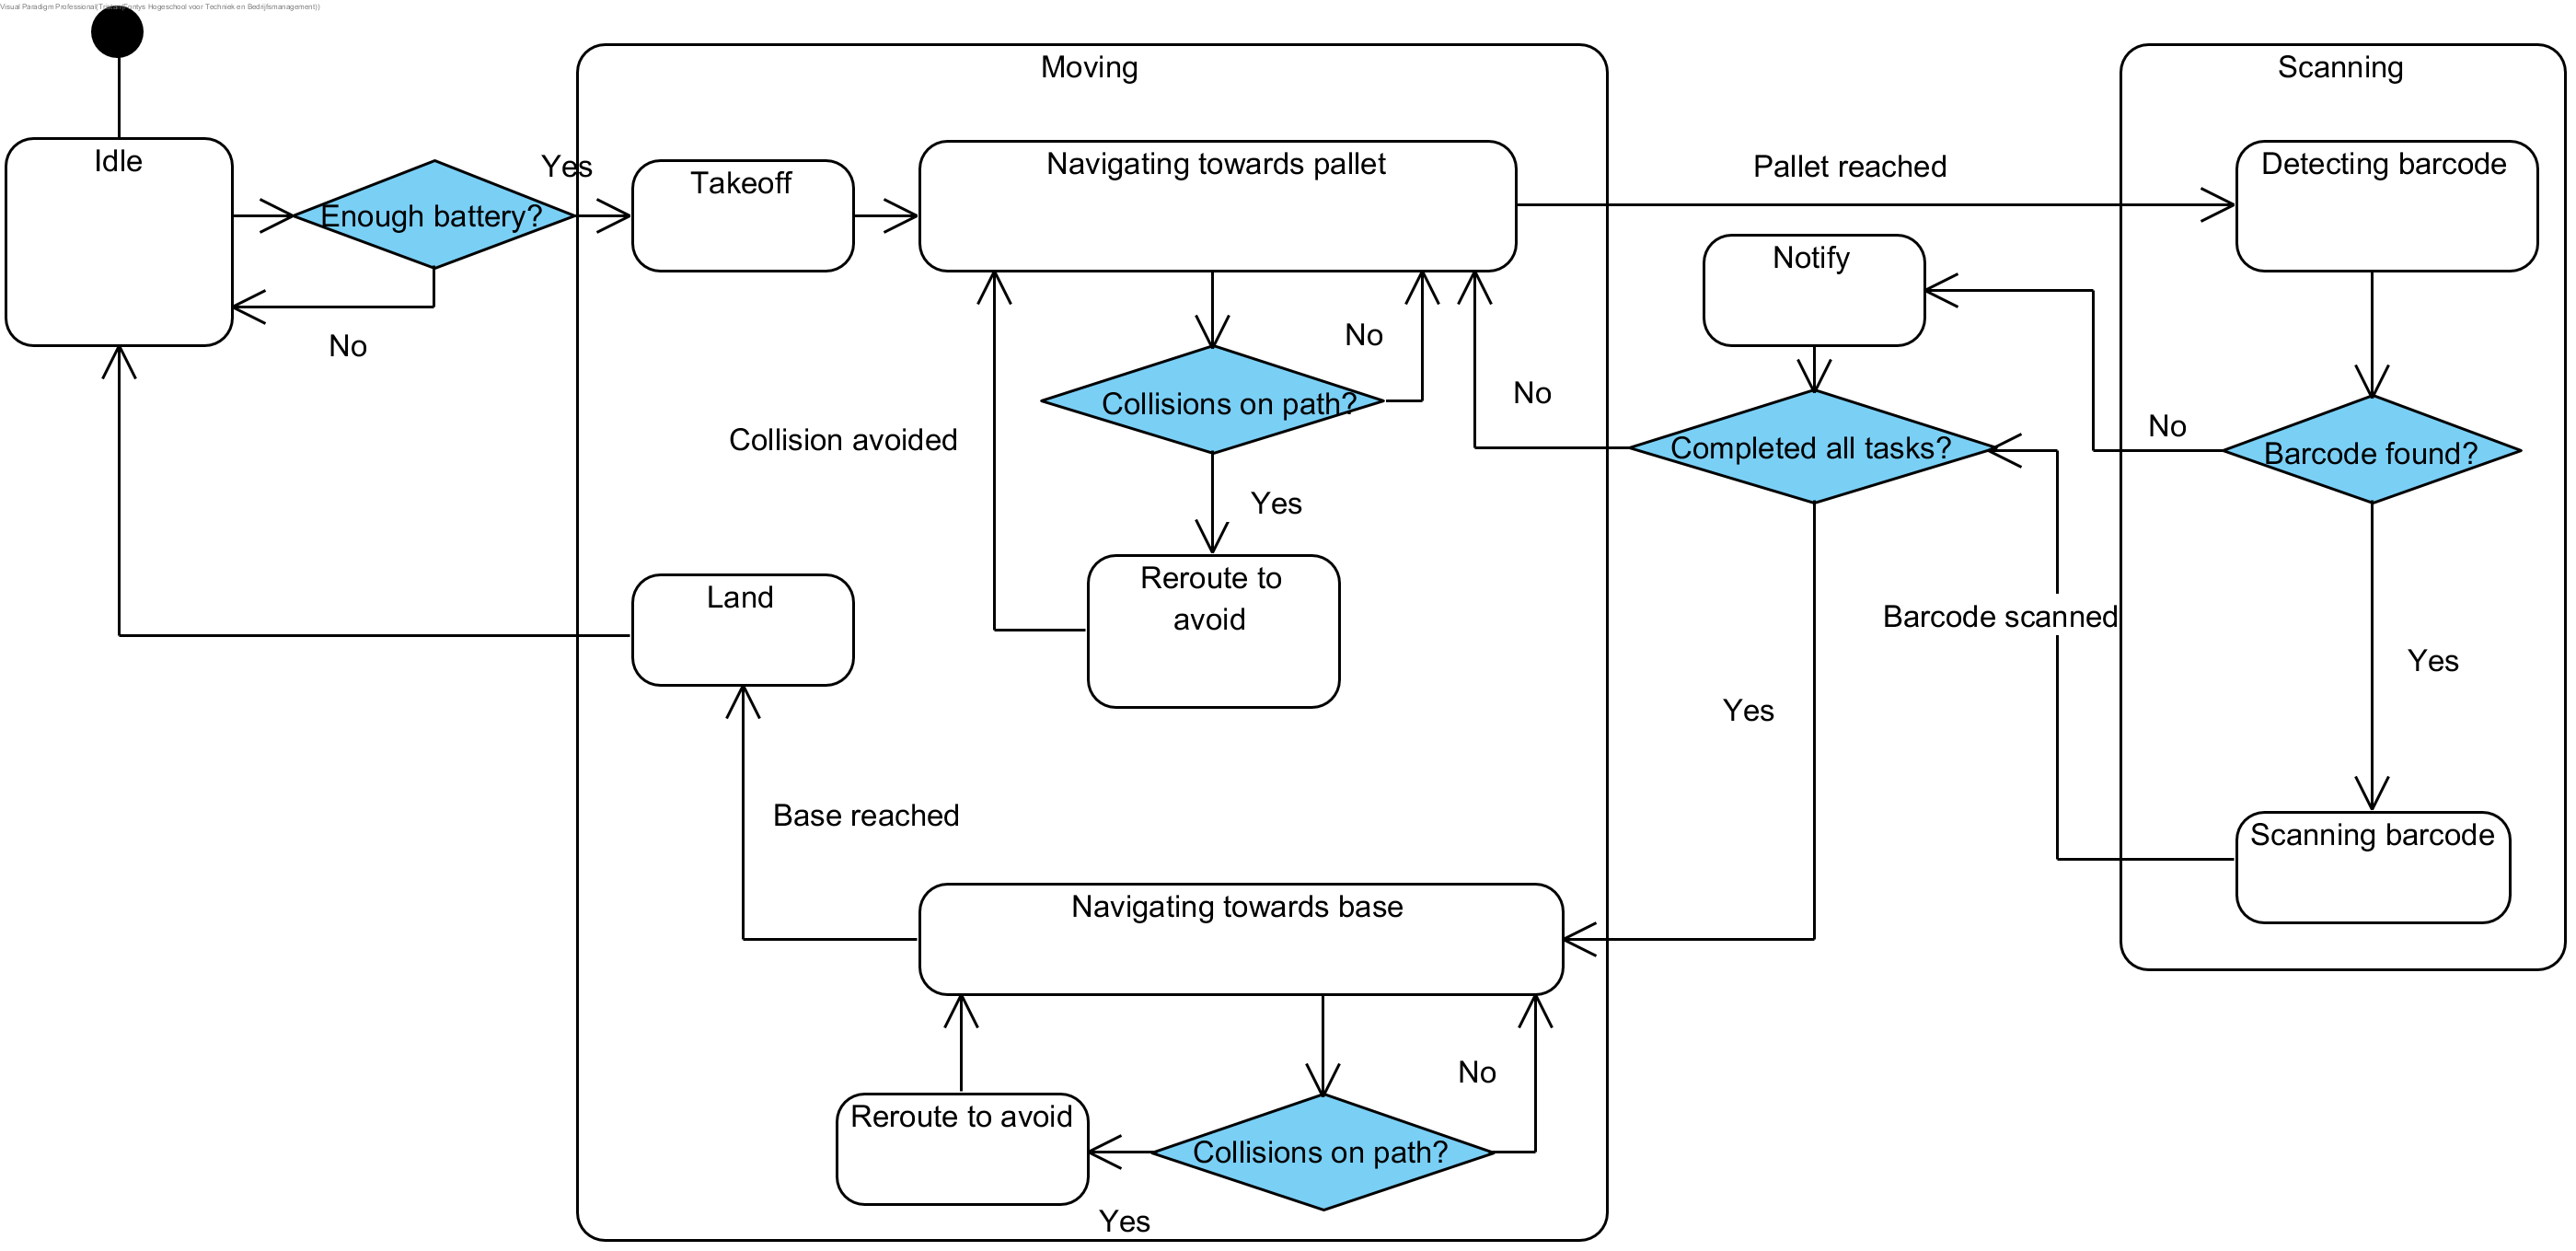
\includegraphics[width=\textwidth, angle=-90]{img/drone_states.png}
	\caption{State model of a drone performing inventory control}
	\label{fig:drone_states}
\end{figure}
	%\end{appendices}
\end{document}